\chapter{Instalando Java}
Trataremos de dar una explicaci\'on de como instalar el lenguaje de programci\'on Java en nuestro sistema operativo, en este caso 
utilizamos Kali, Ubuntu, Windows.

\section{Kali}
En kali linux ya esta instalado, solo falta instalar jdk que se ejecuta con sudo apt install default-jdk ademas el open JDK, para ubuntu especificamos de la siguiente manera
\begin{verbatim}
    javier@javier-Lenovo-G40-80:~$ java --version
    No se ha encontrado la orden «java», pero se puede instalar con:
    sudo apt install default-jre              # version 2:1.11-72build2, or
    sudo apt install openjdk-11-jre-headless  # version 11.0.17+8-1ubuntu2~22.04
    sudo apt install openjdk-17-jre-headless  # version 17.0.5+8-2ubuntu1~22.04
    sudo apt install openjdk-18-jre-headless  # version 18.0.2+9-2~22.04
    sudo apt install openjdk-19-jre-headless  # version 19.0.1+10-1ubuntu1~22.04
    sudo apt install openjdk-8-jre-headless   # version 8u352-ga-1~22.04
\end{verbatim}

\begin{figure}[h!]
    \center
    \begin{minipage}{5cm}
    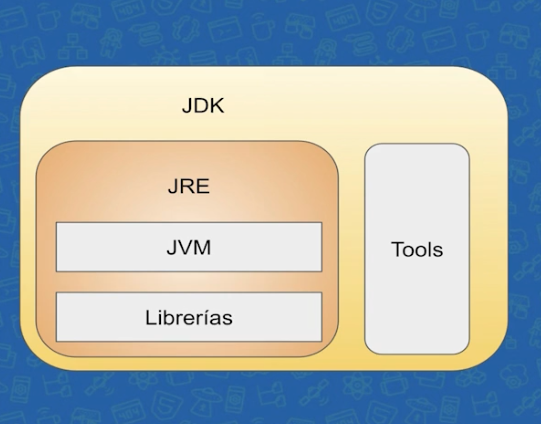
\includegraphics[width=4cm]{Develop/Languages/Java/images/Captura desde 2023-02-08 00-25-57.png}
    \end{minipage}
  \end{figure}


\section{Ubuntu}
\section{Windows}